\documentclass[a4paper, 10pt]{vanvliet_paper}
\usepackage{supertabular}
\usepackage{multicol}
\newacronym{FAS}{fas}{forward association strength}
\newacronym{BAS}{bas}{backward association strength}
\newacronym[\glslongpluralkey={event-related potentials}]{ERP}{erp}{event-related potential}
\newacronym{EEG}{eeg}{electroencephalography}
\newacronym{MEG}{meg}{magnetoencephalography}
\newacronym{EMG}{emg}{electromyography}
\newacronym{EOG}{eog}{electro-oculogram}
\newacronym{MR}{mr}{motor related}
\newacronym{MRP}{mrp}{motor related potential}
\newacronym{RT}{rt}{response time}
\newacronym{LSA}{lsa}{latent semantic analysis}
\newacronym{JAM}{jam}{judgment of associative memory}
\newacronym{BCI}{bci}{brain--computer interface}
\newacronym{LME}{lme}{linear mixed effects}
\newacronym{REML}{reml}{restricted maximum likelihood}
\newacronym{ML}{ml}{maximum likelihood}
\newacronym{ROC}{roc}{receiver operating characteristic}
\newacronym{AUC}{auc}{area under curve}
\newacronym{ROC-AUC}{roc-auc}{receiver operating characteristic -- area under curve}
\newacronym{NS}{ns}{negative slope}
\newacronym{LCMV}{lcmv}{linearly constrained minimum variance}
\newacronym{stLCMV}{\textnormal{st}lcmv}{spatio-temporal linearly constrained minimum variance}
\newacronym[\glslongpluralkey={components of interest}]{COI}{coi}{component of interest}
\newacronym[\glslongpluralkey={regions of interest}]{ROI}{roi}{region of interest}
\newacronym[\glslongpluralkey={generators of interest}]{GOI}{goi}{generator of interest}
\newacronym{ANOVA}{anova}{analysis of variance}
\newacronym{SNR}{snr}{signal-to-noise ratio}
\newacronym{lSVM}{\textnormal{l}svm}{linear support vector machine}
\newacronym{SVM}{svm}{support vector machine}
\newacronym{AoA}{a\textnormal{o}a}{age of acquisition}
\newacronym{PCA}{pca}{principal component analysis}
\newacronym{ICA}{ica}{independent component analysis}
\newacronym{MCMC}{mcmc}{Markov chain Monte Carlo}
\newacronym{LR}{lr}{logistic regression}
\newacronym{LDA}{lda}{linear discriminant analysis}
\newacronym{FC}{fc}{Fisher criterion}
\newacronym{SOA}{soa}{stimulus onset asynchrony}
\newacronym{IIR}{iir}{infinite impulse response}
\newacronym{RVM}{rvm}{random vector model}
\newacronym{RPM}{rpm}{random permutation model}
\newacronym{HAL}{hal}{hyperspace analogue to language}
\newacronym{CAR}{car}{common average reference}
\newacronym{MTG}{mtg}{middle temporal gyrus}
\newacronym{STG}{stg}{superior temporal gyrus}
\newacronym{MTC}{mtc}{medial temporal cortex}
\newacronym{ATC}{atc}{anterior temporal cortex}
\newacronym{AG}{ag}{angular gyrus}
\newacronym{IFG}{ifg}{inferior frontal gyrus}
\newacronym{fMRI}{\textnormal{f}mri}{functional magnetic resonance imaging}
\newacronym{CSP}{csp}{common spatial patterns}
\newacronym{GMM}{gmm}{Guassian mixture model}
\newacronym{OAS}{oas}{oracle approximating shrinkage}
\newacronym{bCSP}{\textnormal{b}csp}{bi-linear common spatial patterns}
\newacronym{HOOI}{hooi}{higher-order orthogonal iteration}
\newacronym{AIC}{aic}{Akaike information criterion}
\newacronym{GLM}{glm}{general linear model}
\newacronym{LARS}{lars}{least-angle regression}
\newacronym{BOLD}{bold}{blood-oxygen level dependant}
\newacronym{SWLDA}{swlda}{step-wise linear discriminant analysis}
\newacronym{OLS}{ols}{ordinary least squares}
\newacronym{SVR}{svr}{support vector regression}
\newacronym{RANSAC}{ransac}{random sample consensus}
\newacronym{MSE}{mse}{mean squared error}
\newacronym{L-BFGS-B}{l-bfgs-b}{Limited-memory Broyden--Fletcher--Goldfarb--Shanno with box constraints}
\newacronym{PDP}{pdp}{parallel distributed processing}
\newacronym{CNN}{cnn}{convolutional neural network}
\newacronym{ReLu}{r\textnormal{e}l\textnormal{u}}{rectified linear unit}
\newacronym{MNE}{mne}{minimum norm estimate}
\newacronym{ECD}{ecd}{equivalent current dipole}

\addbibresource{reading_models.bib}

% Create new LaTeX command \word to typeset literal words in the text (DOGS)
\newcommand{\word}[1]{\textsf{\scriptsize{}#1}}

\draft
\title{A large scale computational model of word recognition and its comparison with MEG data}

\author[1*]{Marijn van Vliet}
\author[1]{Oona Rinkinen}
\author[1]{Takao Shimizu}
\author[2]{Barry Devereux}
\author[1]{Riitta Salmelin}
\affil[1]{Department of Neuroscience and Biomedical Engineering, Aalto University}
\affil[2]{School of Electronics, Electrical Engineering and Computer Science, Queen's University Belfast}
\affil[*]{Corresponding author: marijn.vanvliet@aalto.fi}

\begin{document}
\maketitle

\begin{abstract}
To aid the transition from observation to understanding, we have developed a computational model of word recognition that provides a mechanistic account of how word recognition may be performed in the brain.
This model can accurately identify a bitmap image of rendered text (with arbitrary font-size, font-family and rotation) as one of 10k possible Finnish words.
We show that the model produces activity that mimics that of three evoked components that are observed in \gls{MEG} studies involving the presentation of written words.
\end{abstract}

\section{Introduction}

What computational steps is the brain performing when it recognizes some lines on a piece of paper as a specific word?
This question has been the focus of a large number of neuroimaging studies that examine brain activity during reading.
Noninvasive measurement techniques such as \gls{EEG}\cite{Grainger2009}, \gls{MEG}\cite{Salmelin2007} and \gls{fMRI}\cite{Price2012} have provided a wealth of information about when and where changes in activity might be expected during various tasks involving orthographic processing\cite{Carreiras2014}.
However, these observations alone are unlikely to lead to a complete understanding of the computations performed by the brain during reading\cite{Poeppel2012}.
To develop such an understanding, we need to make these computations explicit, model them, and map the model onto neural signatures observed during imaging studies\cite{Barber2007, Price2018}.
In this study, we introduce a new computational model of visual word recognition that can accurately identify a bitmap image of rendered text (with arbitrary font-size, font-family and rotation) as one of 10k possible Finnish words, while producing activity that can be mapped onto three evoked components that are observed in \gls{MEG} studies involving the presentation of written words.

In the past decades, several computational models have been created that successfully capture some aspects of visual word recognition as performed by the brain.
The \gls{IAC} model of letter perception, by McClelland and Rumelhart\cite{McClelland1981, Rumelhart1982}, was among the first and showed how the interplay of bottom-up and top-down connections results in a system capable of "filling in the blanks" when faced with a partially obscured word.
This model was later extended to model semantics as well, showing how the activation of some semantic features ("is alive", "is a bird") leads to the subsequent activation of more semantic features ("can fly", "lays eggs"), in what became known as the \gls{PDP} framework\cite{McClelland2003}.
As the scope of the models increased, "hand-wiring" the connections in the model became increasingly difficult.
Although \textcite{Coltheart2001} pointed out the benefits of explicitly defined connections in their \gls{DRC} model of visual word recognition and reading out loud, most current models employ back-propagation learn the connections between units based on a large training dataset.
Together, \gls{PDP} and \gls{DRC} models have been shown to account for many behavioral findings, such as reaction times and recognition errors, in both healthy volunteers and patients\cite{McLeod2000, McClelland2003, Perry2007}.
More recently, work has also began to apply these models to explain finding in neuroimaging studies.

\textcite{Laszlo2012} created a \gls{PDP}-style model of visual word recognition that can explain how the computations involved in translating a collection of lines (\word{DOG}) into an abstract semantic representration of a concept (a furry animal that barks).

have shown that by summing the activity of the computational units in specific layers of a \gls{PDP}-style model, the resulting time varying signal resembles a well known signal component, observed in \gls{EEG} and \gls{MEG} studies, known as the N400 potential\cite{Kutas2011}.
This result has later been extended to model more of such components\cite{Laszlo2014}.
However, this 

The original \gls{IAC} model\cite{McClelland1981} defines three levels of perception: the feature level, letter level and word level.
The feature level consists of a "letter bank", in which up to four letters could be loaded, where a single letter is defined as a collection of 16 possible lines.
Each letter bank at the feature level is connected to a group of 26 nodes in the letter level, each node corresponding to a letter, with a line-letter connection indicating that the line was part of the shape of the letter.
Finally, the letter nodes where connected to a large collection of nodes in the word level, each node corresponding to a word, with a letter-word connection indicating that the letter was part of the word.
Note that all connections in this model are well defined and no machine learning is employed in the creation of this model.

Each level consists of a layer of nodes with excitory and inhibitory connections between them, so that activity in one level is propagated to the later levels.


Although the model operates on 5-letter words with an alphabet of only 3 possible letters, \textcite{Laszlo2012} demonstrated how a computational model can both perform a simplified reading task and produce neuroimaging-like data.
However, the signal produced by the model cannot be directly compared with neuroimaging data, because the simulated environment was extremely simplified to reduce the complexity of the model, whereas the brain data will by nature reflect the reading process in a realistic setting.
In fact, none of the existing models of reading can be directly compared to actual neuroimaging data, and it is an often repeated sentiment that there should be more contact between the two\cite{Carreiras2014, Laszlo2012, Laszlo2014, Poeppel2012, Taylor2013}.

Recent advances in deep learning and its software ecosystem are rapidly changing our notion of what is computationally tractable to model\cite{Richards2019}.
\Glspl{CNN} have emerged that perform visual object recognition at a large enough scale to enable a direct comparison between network state and neuroimaging data\cite{Schrimpf2018, Devereux2018, Yamins2016} and consequently our understanding of basic visual processing has increased tremendously\cite{Lindsay2020}.
Since the first stages of reading, namely visual word recognition, can be seen as a specialized form of object recognition, \glspl{CNN} may very well be a suitable tool for increasing the scale of traditional connectionist models of reading.

In this study, we trained a \gls{CNN} to perform visual word recognition on bitmap images of rendered text.
The same set of stimulus images was presented to both the model and human volunteers in order to directly compare the activation inside the model to the amplitude of \gls{MEG} evoked responses recorded from the study participants.
Whereas the training set of the model consisted only of images of either valid Finnish words or only visual noise, the stimulus set used in the experiment contained images of valid Finnish words, which were similar to the ones present in the training data for the model, but also consonant strings, symbol strings and pseudo-words.
We show how various layers in the model behave similarly to several well studied evoked responses and evaluate this similarity both qualitatively and, for the first time, quantitatively.

To aid the transition from observation to understanding, we have developed a computational model of word recognition that is able to operate on the same set of bitmap images used as stimuli in an \gls{MEG} experiment.
This allowed us to directly compare the stimulated with real brain activity.


\section{Results}

\subsection{The brain}

For this study, we reused the \gls{MEG} data that was collected as part of an earlier study by \textcite{Vartiainen2011}.
During the recording session, 15 participants (who gave their informed consent, in agreement with the prior approval of the Helsinki and Uusimaa Ethics Committee) were presented with 560 orthographic stimuli (silent reading task), designed to form a series of experimental contrasts that highlight three processing stages during single word reading.
Stimuli included valid Finnish words, pseudowords, consonant strings, letter-like symbol strings and Finnish words embedded in visual noise (\autoref{fig:stimuli}).

\begin{figure}
    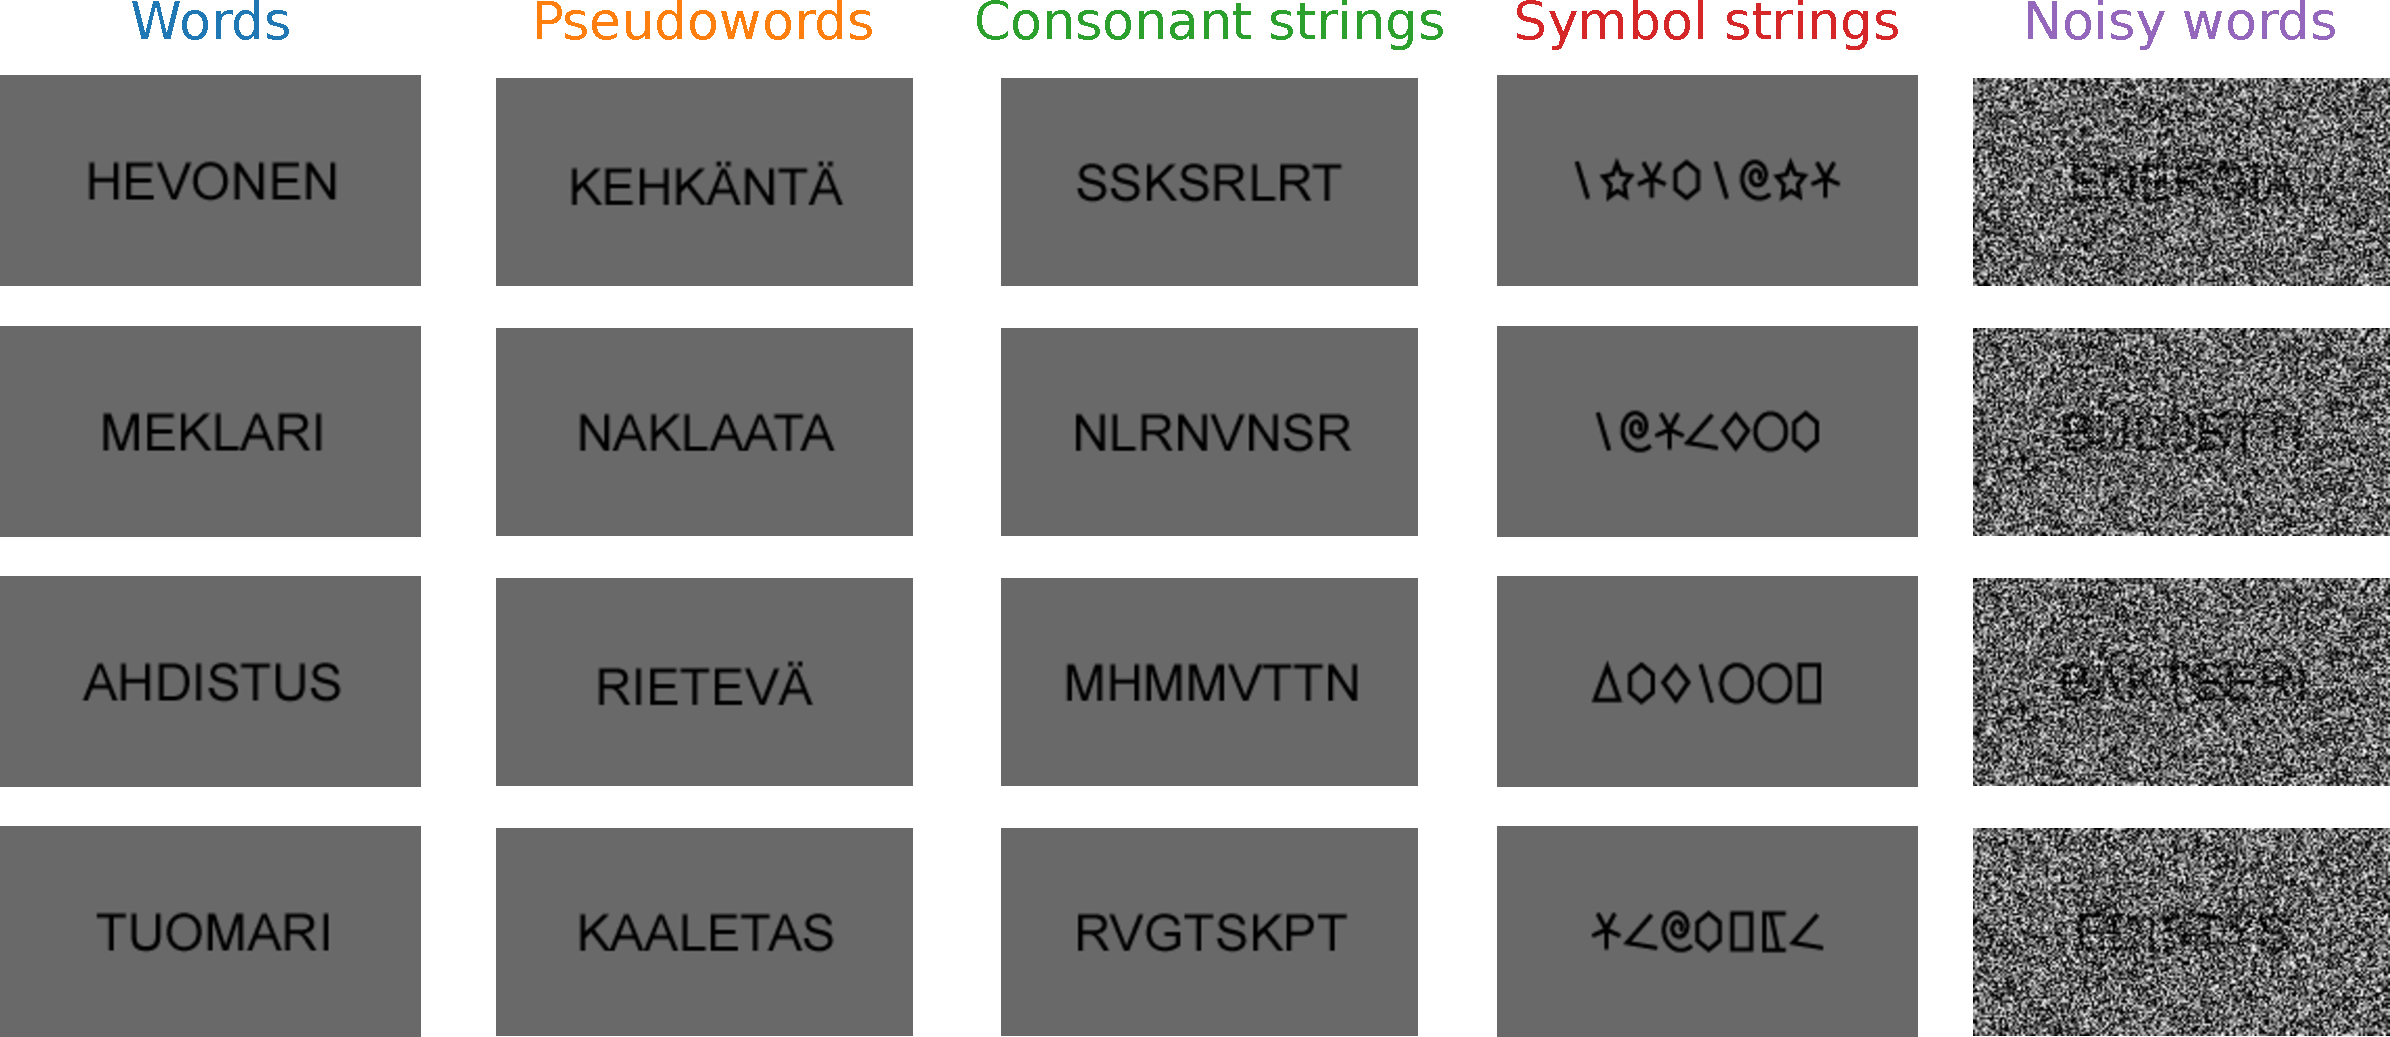
\includegraphics[width=\textwidth]{stimuli.pdf}
    \caption{Examples of stimuli used in the \gls{MEG} experiment. Each stimulus contained 7--8 letters or symbols.}\label{fig:stimuli}
\end{figure}

To summarize the high-dimensional \gls{MEG} data, the sensor level signals were segregated into cortical-level spatiotemporal components by means of guided \gls{ECD} modeling\cite{Hamalainen1993}.
This yielded for each participant, a collection of 11--15 \glspl{ECD} that together account for at least \SI{75}{\percent} of the signal.
The \glspl{ECD} where then grouped based on their location and the timing of peak activation. 
The current study re-uses three of such dipole groups defined in the original study\cite{Vartiainen2011} along the ventral stream (\autoref{fig:results}A), that capture the different processing stages which the experiment sought to highlight.
For each dipole, the response to each stimulus was summarized by integrating the activity over the time window used in \textcite{Vartiainen2011} for statistical analysis.
To obtain the group-level response to each stimulus, the activity integrals for the dipoles in the group were z-transformed across the stimuli, and averaged.

The first group of \glspl{ECD} is occipitally located and is characterized by early onset activity in the visual cortex, peaking \SIrange{65}{115}{\milli\second} after stimulus onset.
The activity at these dipoles is driven by the visual complexity of the stimulus and is characterized in this study by a large response to noise embedded words relative to all other stimulus types.
The second group is located further along the fusiform gyrus, sometimes referred to as the \gls{VWFA}\cite{Cohen2004} and their activity peaks slightly later at \SIrange{140}{200}{\milli\second}.
Dipoles belonging this group exhibit sensitivity to whether the stimulus contains letters that are part of the participant's native alphabet\cite{Tarkiainen1999}, and is characterized in this study by a smaller response to stimuli containing symbol strings and noise embedded words, relative to stimuli that contain letters.
The third and final group is located temporally, peaking much later at \SIrange{300}{500}{\milli\second}, corresponding to the N400 component of the evoked response\cite{Halgren2002, Helenius1998b, Service2007}.
In this group, activity is modulated by the lexical content of the stimulus, and is characterized in this study by a larger response to the word-like (i.e., words and pseudowords) versus the non-word-like stimuli.

\subsection{The model}

As a model of the computations underlying the brain activity observed during the \gls{MEG} experiment, we used a \textsc{VGG}-11\cite{Szegedy2015} network architecture, pretrained on ImageNet\cite{Russakovsky2015}, as provided by the TorchVision package\cite{Marcel2010}.
This architecture consists of five convolution layers (three of which perform convolution twice), followed by two densely connected layers, terminating in an output layer.
The model was trained to perform visual word recognition using a training set that contained 1~000~000 images, where each image depicted one of 10~000 possible Finnish words, rendered in varying fonts, sizes and rotations, with varying degrees of visual background noise (\autoref{fig:train}).
The task for the model was to identify the correct word (by setting the corresponding unit in the output layer to a high value), irregardless of the font, size and rotation used to render the text.
The vocabulary size (10~000) was chosen to exceed the number of units in the densely connected layers (4~096), forcing the model to construct a sub-lexical representation.

\begin{figure}[b]
    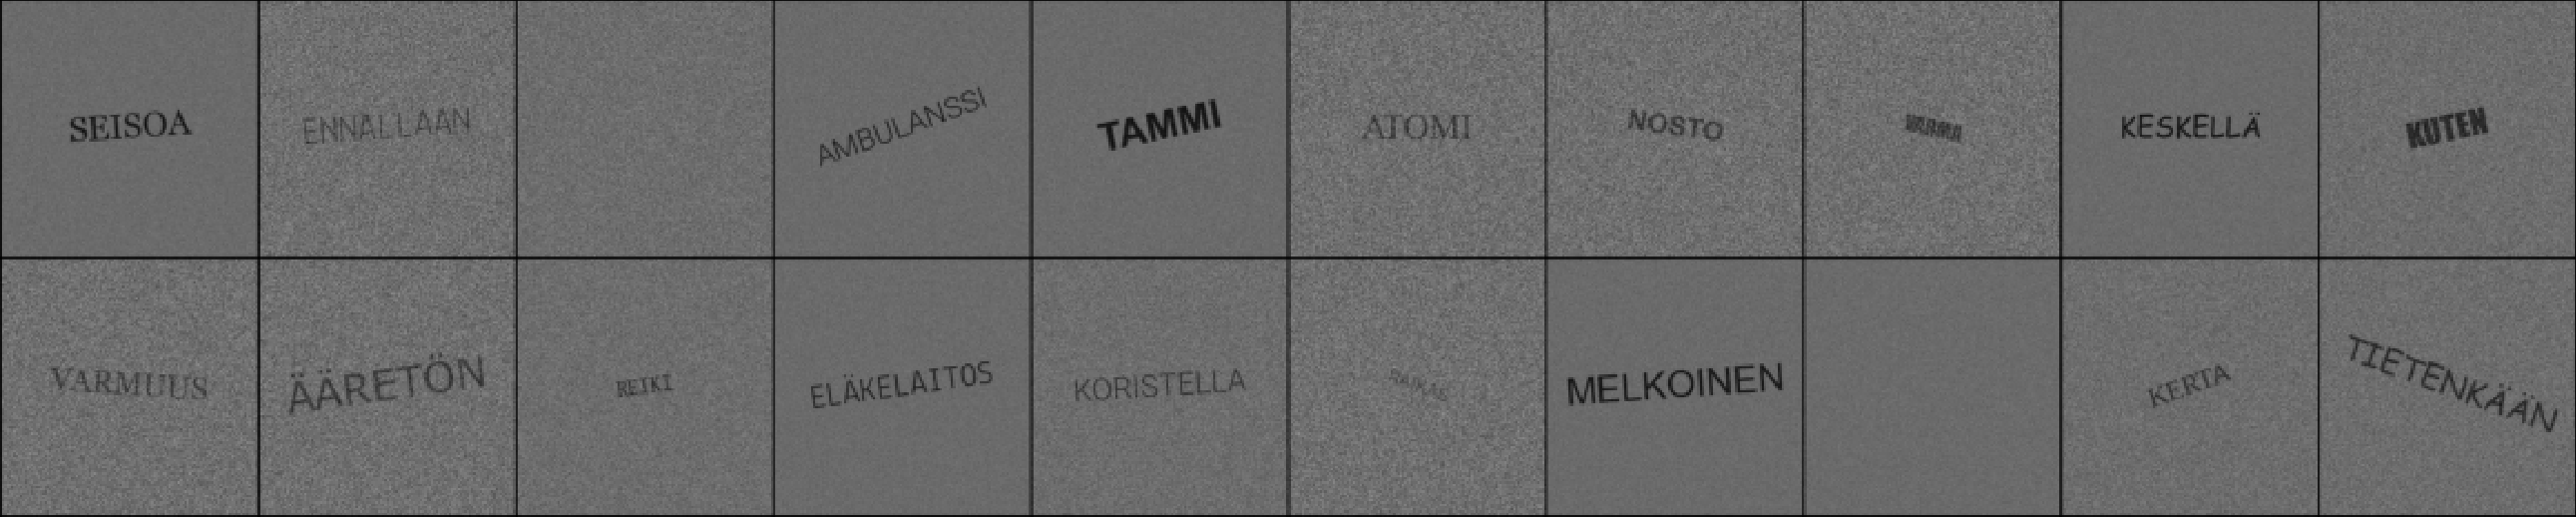
\includegraphics[width=\textwidth]{train.png}
    \caption{Examples of images in the training set for the model.}\label{fig:train}
\end{figure}

In addition to the images of valid Finnish words, 50~000 images consisting of only visual noise were added to the training set.
The inclusion of this "no word present" condition introduces a detection element to what is otherwise a discrimination task.
If no word was present in the image, all output units should have a low value.
%This was achieved by training the model with an additional output unit, indicating the "only noise" condition, while using a cross-entropy loss function, which favors only a single output having a high value, driving all other outputs to zero.
%After training, the final output unit was removed from the model.
During training, the performance of the model was evaluated on an independent test set of 100~000 images that contained words and 5~000 that contained only noise.
Training was stopped when the model's performance plateaued, at which point the accuracy on the test set was \SI{99.3}{\percent}.

After training, the model was used to classify the stimulus images used during the \gls{MEG} experiment (see Supplementary Table 1).
The model classified 113 of the 118 word stimuli correctly (accuracy 95.8\%).
The 5 incorrectly classified stimuli were instead classified as close orthographic neighbours (e.g. LUOMINEN$\rightarrow$TUOMINEN).
All noise embedded words were misclassified, since the amount of noise made them unrecognizable, with 99/118 being classified as the word METSÄTEOLLISUUS, which is one of the words in the training set with the highest visual complexity.
Of course, all the non-word stimuli were misclassified, as the model was not trained on any of these types of stimuli (i.e. pseudowords, consonant strings, symbol strings).
In this case, it was more difficult to find a pattern in the way they were classified.
In many cases, similarity in letter shape seemed to play a role (e.g. SKKNTMT$\rightarrow$SUKUNIMI, ÄHKÄÄJÄ$\rightarrow$VARAAJA), not not always (e.g. TTNRNHR$\rightarrow$UUTINENKIRJE, INKRIHTI$\rightarrow$EMOLEVY).


\subsection{Comparing model and brain}

To directly compare layer activations in the model to dipole responses in the brain (\autoref{fig:results}, middle), the sum activation in each layer of the model was recorded for each stimulus as it passed through the model (\autoref{fig:results}B).
Since the same stimuli were processed by both the model and the brain, we can measure the model-brain correspondence qualitatively by examining the responses to each stimulus type, and quantitatively by computing the correlation between the summarized activity in the model layers and dipole groups (\autoref{tab:correlations}).

\begin{table}[b]
    \begin{tabular}{rlrrr}
        \toprule
        Layer & Type        & Dipole group 1 & Dipole group 2 & Dipole group 3 \\
        \midrule
            1 & Convolution &           0.79 &          -0.48 &          -0.35 \\
            2 & Convolution &           0.79 &          -0.48 &          -0.35 \\
            3 & Convolution &           0.68 &          -0.42 &          -0.33 \\
            4 & Convolution &           0.15 &          -0.03 &          -0.01 \\
            5 & Convolution &           0.66 &          -0.32 &          -0.19 \\
            6 & Fully conn. &          -0.32 &           0.39 &           0.39 \\
            7 & Fully conn. &          -0.53 &           0.47 &           0.43 \\
            8 & Output      &          -0.61 &           0.45 &           0.44 \\
        \bottomrule
    \end{tabular}
    \caption{Pearson correlations between each layer of the model and the grand-average of each dipole group.}\label{tab:correlations}
\end{table}

In the first three convolution layers of the model, we see a much larger response to the "noisy word" stimuli, relative to the other stimulus types, likely driven by the much higher visual complexity of these stimuli.
Convolution filters that are detecting edges and corners output high values for visual noise and low values for stretches of flat gray background.
This corresponds well to the response of the first dipole group (Pearson correlations: 0.79, 0.79, 0.68), localized in the visual cortex of the brain, which shows a similar sensitivity to noise, and does not distinguish between the other stimulus types.

We see a change in the response pattern of the model in the next two convolution layers: layers 4 and 5.
In these layers, the activity in response to symbol strings is now lower than that of the other types.
This indicates the presence of convolution filters that are sensitive to the specific line arrangements that are found in letters of the Finnish alphabet, which are not present in the symbol strings.
In this regard, these layers correspond to the responses of dipole group two in the brain.
However, many of the filters are still sensitive to noise, which does not correspond to the responses of the second dipole group, resulting in a negative correlation (Pearson correlations: -0.03, -0.32).
Overall, layers 4 and 5 correspond best to dipole group one (Pearson correlations: 0.15, 0.66).

The selectivity for letter shapes becomes more pronounced in the two fully connected layers of the model.
In these layers, we also see less activity in response to the noise stimuli.
However, no distinction is made between consonant strings and word-like stimuli, indicating that letters are detected in isolation.
This means the response patterns of these layers correspond to that of the second dipole group (Pearson correlations 0.39, 0.47).

Finally, at the output layer of the model, we observe that consonant strings produce less activity, indicating that the shapes of multiple letters are combined to produce the output.
It is noteworthy that pseudowords, which were not present in the training set, produce a roughly equal amount of activation in the output layer as valid Finnish words.
This means that the response pattern of the output layer corresponds to that of the third dipole group (Pearson correlation 0.44).

\begin{figure*}
    \includegraphics[width=18cm]{results.pdf}
    \vspace{2ex}
    \caption{
        \textbf{Comparison between \gls{MEG} evoked activity and sum activity in each layer of the model.}
        Based on the response pattern to each stimulus type, three processing stages where identified that correspond to different time windows in the \gls{MEG} activity and different layer types in the model.\\
        \textbf{A)} Evoked \gls{MEG} activity, quantified during three time intervals.
        The grand-average \gls{MNE} source activity to valid Finnish words is shown in orange hues.
        Overlaid are the positions of the most representative \gls{ECD} for each participant during the indicated time interval, as determined by \textcite{Vartiainen2011}.
        Below is shown for each stimulus, the grand-average activity at the \glspl{ECD}, integrated over the indicated time interval.\\
        \textbf{B)} For each layer of the model, the sum \gls{ReLu} activation in each layer in response to each stimulus.
        The network architecture is shown below.
    }\label{fig:results}
\end{figure*}

\section{Discussion}
One may ask why the lexicon layer of the model is a one-hot encoded output vector.
This is plainly incompatible with how the brain works.
Some abstract semantic representation, such as word2vec or semantic features would clearly be better candidates.
The reason why the final layer of the model is the way it is, is because this is the point where a hard 90 degree turn needs to be made from orthographic similarity to semantic similarity.

The model used in this study is a standard convolutional design and has many shortcomings as a model of the brain.
Nevertheless, the fact that the model performs well despite these shortcomings shows the power of using deep learning models to implement cognitive theories.

\section{Methods}
\section{Acknowledgements}
We acknowledge the computational resources provided by the Aalto Science-IT project.
This research was funded by the Academy of Finland (grant \#310988 to M.v.V, \#255349, \#256459, \#283071 and \#315553 to R.S.).
% TODO: Barry funding information

\newpage
\printbibliography{}

\end{document}
